%%%%%%%%%%%%%%%%%%%%%%%%%%%%%%%%%%%%%%%%%%%%%%%%%%%%%%%%%%%%%%%%%%%%%%%
% NOTE: Add the following to your main document preamble:
%
% \usepackage{xcolor}
% \usepackage{tcolorbox}
% \tcbuselibrary{skins,breakable}
% \usepackage{tikz}
% \usepackage{fontawesome5}
% \usepackage{booktabs}
%
\definecolor{headerblue}{RGB}{41, 128, 185}
\definecolor{metricgreen}{RGB}{39, 174, 96}
\definecolor{alertred}{RGB}{192, 57, 43}
\definecolor{warningyellow}{RGB}{243, 156, 18}
\definecolor{lightblue}{RGB}{240, 245, 255}
\definecolor{darkblue}{RGB}{30, 60, 120}
\definecolor{mutationpurple}{RGB}{142, 68, 173}
\definecolor{crossoverblue}{RGB}{52, 152, 219}
%
%%%%%%%%%%%%%%%%%%%%%%%%%%%%%%%%%%%%%%%%%%%%%%%%%%%%%%%%%%%%%%%%%%%%%%%

\section{Case Study: Factor Evolution Trajectory}
\label{sec:appendix_case_study}

This appendix presents a detailed case study of factor evolution in QuantaAlpha. We trace the complete trajectory of a representative factor---\textit{Institutional\_Momentum\_Score\_20D}---through the crossover phase, demonstrating how the evolutionary framework synthesizes complementary market hypotheses from parent trajectories.

QuantaAlpha's evolution process operates in three phases: (1) \textbf{Original} phase where initial hypotheses are generated, (2) \textbf{Mutation} phase where existing trajectories are perturbed to explore orthogonal strategies, and (3) \textbf{Crossover} phase where high-performing parent trajectories are combined to synthesize offspring with potentially superior predictive power. The following factor card illustrates a Round 8 Crossover operation.

%%%%%%%%%%%%%%%%%%%%%%%%%%%%%%%%%%%%%%%%%%%%%%%%%%%%%%%%%%%%%%%%%%%%%%%
% Factor Identity Card
%%%%%%%%%%%%%%%%%%%%%%%%%%%%%%%%%%%%%%%%%%%%%%%%%%%%%%%%%%%%%%%%%%%%%%%
\subsection{Factor Identity}

The factor card below presents the basic information of the evolved factor, including its unique identifiers, evolution lineage, and mathematical formulation.

\begin{tcolorbox}[
  colback=lightblue,
  colframe=darkblue,
  fonttitle=\bfseries,
  title={\faTag\ Institutional\_Momentum\_Score\_20D},
  arc=2mm,
  boxrule=0.5pt,
  breakable
]

\begin{tabular}{@{}ll@{}}
\textbf{Factor ID:} & \texttt{c57cace576a95356} \\
\textbf{Trajectory ID:} & \texttt{df5a496878f4} \\
\textbf{Evolution Round:} & Round 8 \\
\textbf{Evolution Phase:} & \colorbox{crossoverblue!20}{\textcolor{crossoverblue}{\textbf{Crossover}}} \\
\textbf{Direction ID:} & 6 \\
\end{tabular}

\vspace{0.3cm}

\textbf{Factor Expression:}
\begin{tcolorbox}[colback=darkblue!5, colframe=darkblue, boxrule=0.3pt, arc=1mm]
\small\ttfamily
RANK(TS\_CORR(DELTA(close, 1)/close, DELTA(volume, 1)/volume, 20) * TS\_MEAN((close - open)/close, 5))
\end{tcolorbox}

\textbf{Mathematical Formulation:}
\[
\text{IMS}_{20D} = \text{RANK}\left(\rho_{20}\left(\frac{\Delta P}{P}, \frac{\Delta V}{V}\right) \times \overline{\left(\frac{C - O}{C}\right)}_{5}\right),
\]
\small
where $\rho_{20}(\cdot,\cdot)$ denotes the 20-day rolling correlation, $\Delta P/P$ is the daily return, $\Delta V/V$ is the volume change ratio, $\overline{(\cdot)}_5$ is the 5-day moving average, and $C$ and $O$ represent the closing and opening prices, respectively.

\vspace{0.2cm}

\textbf{Factor Interpretation:}\\
\small
This factor captures institutional-driven momentum by measuring two key signals: (1) the correlation between price returns and volume changes, which indicates coordinated institutional trading when positive; and (2) the average intraday return pattern, reflecting institutional activity that typically influences closing prices. The cross-sectional ranking ensures comparability across stocks.

\end{tcolorbox}

%%%%%%%%%%%%%%%%%%%%%%%%%%%%%%%%%%%%%%%%%%%%%%%%%%%%%%%%%%%%%%%%%%%%%%%
% Evolution Lineage
%%%%%%%%%%%%%%%%%%%%%%%%%%%%%%%%%%%%%%%%%%%%%%%%%%%%%%%%%%%%%%%%%%%%%%%
\subsection{Evolution Lineage}

The crossover operation combines insights from two parent trajectories with complementary market hypotheses. Parent 1 focuses on identifying \textit{fragile momentum} driven by retail speculation, while Parent 2 targets \textit{sustainable momentum} supported by institutional activity. The LLM synthesizes these complementary perspectives into a unified framework.

\begin{tcolorbox}[
  colback=lightblue,
  colframe=darkblue,
  fonttitle=\bfseries,
  title={\faDna\ Evolution Information},
  arc=2mm,
  boxrule=0.5pt,
  breakable
]

\textbf{\faCodeBranch\ Parent Trajectories:}

\vspace{0.3cm}

\begin{tcolorbox}[colback=lightblue, colframe=darkblue!50, boxrule=0.3pt, title={\small\textbf{Parent 1: 1e6d57e38e89}}, fonttitle=\bfseries\small]
\small
\begin{tabular}{@{}ll@{}}
\textbf{Round:} & Round 7 \\
\textbf{Phase:} & Mutation \\
\textbf{Rank IC:} & 0.0216 \\
\textbf{IC:} & 0.0059 \\
\textbf{IR:} & 1.297 \\
\end{tabular}

\vspace{0.2cm}
\textbf{Core Hypothesis:}\\
\small
When retail investors exhibit herd behavior and momentum chasing in stocks with high social media activity, but accompanied by declining institutional ownership and deteriorating fundamentals, the resulting price momentum is unsustainable and leads to mean reversion.
\end{tcolorbox}

\vspace{0.2cm}

\begin{tcolorbox}[colback=lightblue, colframe=darkblue!50, boxrule=0.3pt, title={\small\textbf{Parent 2: 47e0f0e55382}}, fonttitle=\bfseries\small]
\small
\begin{tabular}{@{}ll@{}}
\textbf{Round:} & Round 6 \\
\textbf{Phase:} & Crossover \\
\textbf{Rank IC:} & 0.0246 \\
\textbf{IC:} & 0.0069 \\
\textbf{IR:} & 1.347 \\
\end{tabular}

\vspace{0.2cm}
\textbf{Core Hypothesis:}\\
\scmall
A regime-adaptive structural momentum factor combining institutional ownership-driven medium-term price trends with short-term microstructure regime validation, where coordinated accumulation/distribution patterns amplify momentum when confirmed by microstructure alignment.
\end{tcolorbox}

\vspace{0.3cm}

\textbf{\faSitemap\ Evolution Path Diagram:}
\begin{center}
\resizebox{0.7\linewidth}{!}{%
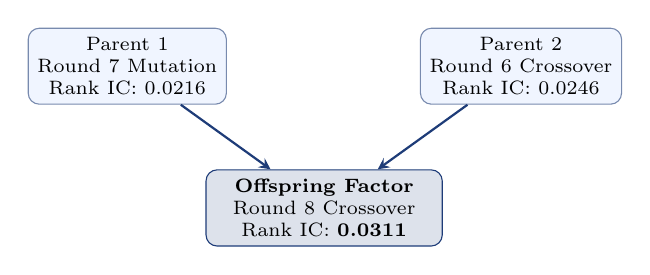
\begin{tikzpicture}[
    node distance=1.5cm,
    roundbox/.style={rectangle, rounded corners, align=center, font=\scriptsize},
    parentbox/.style={roundbox, draw=darkblue!60, fill=lightblue, minimum width=2.5cm, minimum height=0.8cm},
    childbox/.style={roundbox, draw=darkblue, fill=darkblue!15, minimum width=3cm},
    arrow/.style={->, thick, >=stealth, color=darkblue}
]
    % Parent nodes
    \node[parentbox] (p1) at (-2.5, 1.8) {Parent 1\\Round 7 Mutation\\Rank IC: 0.0216};
    \node[parentbox] (p2) at (2.5, 1.8) {Parent 2\\Round 6 Crossover\\Rank IC: 0.0246};
    
    % Current node
    \node[childbox] (current) at (0, 0) {\textbf{Offspring Factor}\\Round 8 Crossover\\Rank IC: \textbf{0.0311}};
    
    % Arrows
    \draw[arrow] (p1) -- (current);
    \draw[arrow] (p2) -- (current);
    
    % Label
\end{tikzpicture}%
}
\end{center}

\end{tcolorbox}

%%%%%%%%%%%%%%%%%%%%%%%%%%%%%%%%%%%%%%%%%%%%%%%%%%%%%%%%%%%%%%%%%%%%%%%
% Synthesized Hypothesis
%%%%%%%%%%%%%%%%%%%%%%%%%%%%%%%%%%%%%%%%%%%%%%%%%%%%%%%%%%%%%%%%%%%%%%%
\subsection{Synthesized Hypothesis}

Through crossover, the LLM generates a new hypothesis that integrates the complementary insights from both parents, rather than simply averaging their factor expressions. This hypothesis-driven approach ensures that the offspring factor captures genuinely novel market dynamics.

\begin{tcolorbox}[
  colback=lightblue,
  colframe=darkblue,
  fonttitle=\bfseries,
  title={\faLightbulb\ Hypothesis},
  arc=2mm,
  boxrule=0.5pt,
  breakable
]

\textbf{Core Hypothesis:}\\
A regime-aware dual-source momentum factor that combines institutional-driven structural momentum (validated by healthy microstructure) and retail-driven speculative momentum (characterized by high attention and deteriorating fundamentals), dynamically weighted by market volatility: amplifying institutional signals in stable regimes and retail reversal signals in turbulent regimes, will generate superior predictive returns.

\vspace{0.3cm}

\begin{tabular}{@{}p{0.28\textwidth}p{0.67\textwidth}@{}}
\toprule
\textbf{Component} & \textbf{Description} \\
\midrule
\textbf{Observation} & Parent strategies separately targeting institutional trends and retail herding show moderate predictive power (Rank IC $\sim$0.02--0.025), suggesting combined signals could capture complementary market dynamics. \\
\midrule
\textbf{Justification} & Sustainable price trends require institutional sponsorship and orderly trading, while retail-driven bubbles lack fundamental support and reverse under stress; a hybrid model exploiting both can enhance robustness across market regimes. \\
\midrule
\textbf{Domain Knowledge} & Institutional accumulation with strong price-volume correlation and low volatility indicates sustainable momentum; retail herding with declining institutional ownership and high volatility signals fragile momentum prone to reversal. \\
\bottomrule
\end{tabular}

\end{tcolorbox}

%%%%%%%%%%%%%%%%%%%%%%%%%%%%%%%%%%%%%%%%%%%%%%%%%%%%%%%%%%%%%%%%%%%%%%%
% Backtest Results
%%%%%%%%%%%%%%%%%%%%%%%%%%%%%%%%%%%%%%%%%%%%%%%%%%%%%%%%%%%%%%%%%%%%%%%
\subsection{Backtest Performance}

After factor construction, QuantaAlpha automatically backtests the generated factors using the Qlib framework. The results below compare the offspring factor against both parent trajectories and the baseline, demonstrating the effectiveness of the crossover operation.

\begin{tcolorbox}[
  colback=lightblue,
  colframe=darkblue,
  fonttitle=\bfseries,
  title={\faChartLine\ Backtest Metrics},
  arc=2mm,
  boxrule=0.5pt,
  breakable
]

\begin{center}
\begin{tabular}{@{}lccc@{}}
\toprule
\textbf{Metric} & \textbf{Offspring Factor} & \textbf{Baseline} \\
\midrule
\textbf{IC} & 0.0126 & 0.0058 \\
\textbf{Rank IC} & \textbf{0.0311} & 0.0220 \\
\midrule
\textbf{ARR (Excess)} & 7.80\% & 5.20\% \\
\textbf{IR} & 0.963 & 0.973 \\
\textbf{MDD (Excess)} & $-$11.37\% & $-$7.30\% \\
\bottomrule
\end{tabular}
\end{center}

\vspace{0.3cm}

\textbf{Detailed Statistics:}
\begin{center}
\small
\begin{tabular}{@{}ll|ll@{}}
\toprule
\textbf{Metric} & \textbf{Value} & \textbf{Metric} & \textbf{Value} \\
\midrule
\textbf{Daily Excess Return (w/o cost)} & 0.0328\% & \textbf{Daily Excess Return (w/ cost)} & 0.0128\% \\
\textbf{Excess Return Std} & 0.52\% & \textbf{Turnover (FFR)} & 100\% \\
\textbf{L2 Train Loss} & 0.9936 & \textbf{L2 Valid Loss} & 0.9962 \\
\bottomrule
\end{tabular}
\end{center}

\end{tcolorbox}

%%%%%%%%%%%%%%%%%%%%%%%%%%%%%%%%%%%%%%%%%%%%%%%%%%%%%%%%%%%%%%%%%%%%%%%
% LLM Feedback
%%%%%%%%%%%%%%%%%%%%%%%%%%%%%%%%%%%%%%%%%%%%%%%%%%%%%%%%%%%%%%%%%%%%%%%
\subsection{LLM Feedback and Iteration Guidance}

After evaluating backtest results, the LLM provides structured feedback that guides subsequent evolution rounds. This feedback loop enables continuous improvement by learning from both successes and failures.

\begin{tcolorbox}[
  colback=lightblue,
  colframe=darkblue,
  fonttitle=\bfseries,
  title={\faComments\ Feedback \& Evaluation},
  arc=2mm,
  boxrule=0.5pt,
  breakable
]

\textbf{\faSearch\ Observations:}\\
The crossover operation demonstrates a trade-off between enhanced predictive accuracy and increased risk exposure compared to the baseline:
\begin{itemize}
    \item \textcolor{metricgreen}{\faCheckCircle} Significant improvement in annualized excess return and predictive metrics (IC and Rank IC), validating the effectiveness of synthesizing dual-source momentum signals.
    \item \textcolor{alertred}{\faTimesCircle} Increased maximum drawdown and a marginal decline in the Information Ratio, suggesting that the offspring factor introduces higher volatility during certain market regimes.
\end{itemize}

\vspace{0.2cm}

\textbf{\faBalanceScale\ Hypothesis Evaluation:}\\[0.15cm]
\small
Results partially support the hypothesis. Improved annualized return and IC suggest that combining institutional and retail momentum signals has merit. However, deterioration in risk metrics indicates that without proper regime-adaptive weighting, the combined signals may amplify risks during turbulent periods. The full hypothesis requires all three components (institutional momentum, retail herding reversal, volatility-adaptive weighting) to work effectively.

\vspace{0.2cm}

\textbf{\faFlag\ Decision:} \colorbox{alertred!20}{\textcolor{alertred}{\textbf{REJECTED}}} for direct deployment.

\vspace{0.2cm}

\textbf{\faExclamationTriangle\ Recommendations for Next Iteration:}
\begin{enumerate}
    \setlength{\itemsep}{0pt}
    \setlength{\parsep}{0pt}
    \setlength{\topsep}{0pt}
    \setlength{\partopsep}{0pt}
    \small
    \item Use 20-day price-volume correlation as institutional momentum proxy;
    \item Use 5-day average intraday returns as retail attention proxy;
    \item Add volatility regime indicator (recent/historical volatility ratio) for dynamic weighting.
\end{enumerate}

\small This feedback will inform the next mutation round, guiding the LLM to simplify the factor expression while preserving the core dual-source concept.

\end{tcolorbox}

%%%%%%%%%%%%%%%%%%%%%%%%%%%%%%%%%%%%%%%%%%%%%%%%%%%%%%%%%%%%%%%%%%%%%%%%%%%%%%
%%%%%%%%%%%%%%%%%%%%%%%%%%%%%%%%%%%%%%%%%%%%%%%%%%%%%%%%%%%%%%%%%%%%%%%%%%%%%%